\documentclass[a4paper, 11pt, twoside]{article}

\usepackage{hyperref}
%\usepackage[ngerman]{babel}
\usepackage[english]{babel}
%\usepackage[latin1]{inputenc}
\usepackage[utf8]{inputenc}

\usepackage{graphicx,float,subfigure}
%\usepackage{pifont}
\usepackage{type1cm}
\usepackage{amssymb, amsthm, amsmath}
\usepackage{listings}

\usepackage{algorithm}
\usepackage{algpseudocode}
\usepackage{tikz}


\usepackage{pgf}
\usepackage{url}
%\usepackage{graphicx}
%\usepackage{pifont}
%\usepackage{type1cm}


\usepackage{makeidx}
\makeindex

\setlength{\parindent}{0em}
\setlength{\oddsidemargin}{0.0cm}
\setlength{\evensidemargin}{0.0cm}
\setlength{\textheight}{23cm}
\setlength{\topmargin}{-0.5cm}
\setlength{\footskip}{1.5cm}
\setlength{\textwidth}{15.5cm}

\renewcommand*\familydefault{\sfdefault}

\begin{document}
\thispagestyle{empty}

%\documentclass[a4paper]{article}

%\usepackage{pgf}
%\usepackage{graphicx}
%\usepackage{pifont}
%\usepackage{type1cm}

\setlength{\textwidth}{14cm}
\setlength{\oddsidemargin}{1cm}

%\begin{document}

\thispagestyle{empty}

%%%%%%%%%%%%%%%%%%%%%%%%%%%%%%%%%%%%%%%%
%%%%%%%%%%%%%%%%%%%%%%%%%%%%%%%%%%%%%%%%
%%%%%%%%%%%%%%%%%%%%%%%%%%%%%%%%%%%%%%%%

\newcount \Z
\Z=20

%%% logos %%%

%%% NUMHPC %%%
\newlength{\numhpclogox}
\setlength{\numhpclogox}{\paperwidth} % 20/210ths of the paperwidth
\divide\numhpclogox by 210
\multiply\numhpclogox by 100

\newlength{\numhpclogoy}
\setlength{\numhpclogoy}{\paperheight} % 270/297ths of the paperwidth
\divide \numhpclogoy by 297
\multiply \numhpclogoy by -235

\newlength{\numhpclogoheight}
\setlength{\numhpclogoheight}{\paperheight} % 270/297ths of the paperwidth
\divide\numhpclogoheight by 297
\multiply\numhpclogoheight by 20

%%% KIT %%%
\newlength{\kitlogox}
\setlength{\kitlogox}{\paperwidth} % 20/210ths of the paperwidth
\divide\kitlogox by 210
\multiply\kitlogox by 0

\newlength{\kitlogoy}
\setlength{\kitlogoy}{\paperheight} % 270/297ths of the paperwidth
\divide \kitlogoy by 297
\multiply \kitlogoy by -230

\newlength{\kitlogoheight}
\setlength{\kitlogoheight}{\paperheight} % 270/297ths of the paperwidth
\divide\kitlogoheight by 297
\multiply\kitlogoheight by 15


%%% EMCL %%%
\newlength{\emcllogox}
\setlength{\emcllogox}{\paperwidth} % 20/210ths of the paperwidth
\divide\emcllogox by 210
\multiply\emcllogox by 28

\newlength{\emcllogoy}
\setlength{\emcllogoy}{\paperheight} % 270/297ths of the paperwidth
\divide \emcllogoy by 297
\multiply \emcllogoy by -160

\newlength{\emcllogoheight}
\setlength{\emcllogoheight}{\paperheight} % 270/297ths of the paperwidth
\divide\emcllogoheight by 297
\multiply\emcllogoheight by 20

%%% HIFLOW %%%
\newlength{\hiflowlogox}
\setlength{\hiflowlogox}{\paperwidth} % 20/210ths of the paperwidth
\divide\hiflowlogox by 210
\multiply\hiflowlogox by 28

\newlength{\hiflowlogoy}
\setlength{\hiflowlogoy}{\paperheight} % 270/297ths of the paperwidth
\divide \hiflowlogoy by 297
\multiply \hiflowlogoy by -160

\newlength{\hiflowlogoheight}
\setlength{\hiflowlogoheight}{\paperheight} % 270/297ths of the paperwidth
\divide\hiflowlogoheight by 297
\multiply\hiflowlogoheight by 33

%%%%%%%%%%%%%%%%%%%%%%%%%%%%%%%%%%%%%%%%
%%%%%%%%%%%%%%%%%%%%%%%%%%%%%%%%%%%%%%%%
%%%%%%%%%%%%%%%%%%%%%%%%%%%%%%%%%%%%%%%%

%%% NUMHPC %%%
%%\pgftext[bottom, left, at={\pgfpointadd{\pgfpoint{0pt}{0pt}}{\pgfpoint{\numhpclogox}{\numhpclogoy}}}]{\includegraphics[totalheight=\numhpclogoheight]{numhpc}}

%%% KIT %%%
%%\pgftext[bottom, left, at={\pgfpointadd{\pgfpoint{0pt}{0pt}}{\pgfpoint{\kitlogox}{\kitlogoy}}}]{\includegraphics[totalheight=\kitlogoheight]{kitlogo}}

%%% EMCL %%%
\pgftext[bottom, left, at={\pgfpointadd{\pgfpoint{0pt}{0pt}}{\pgfpoint{\hiflowlogox}{\hiflowlogoy}}}]{
\includegraphics[totalheight=\hiflowlogoheight]{HF3_color}}

%%% horizontal lines %%%
\pgfline{\pgfxy(-1pt,0.1pt)}{\pgfxy(15pt,0.1pt)}
\pgfline{\pgfxy(-1pt,-21.4pt)}{\pgfxy(15pt,-21.4pt)}
%%\pgfline{\pgfxy(-1pt,-22.4pt)}{\pgfxy(15pt,-22.4pt)}

%%% EMCL text %%%
\pgftext[bottom, left, at={\pgfpointadd{\pgfpoint{0pt}{0pt}}{\pgfpoint{0cm}{1cm}}}]{{\LARGE{{\bf Tutorial}}}}

%%% EMCL web %%%
\pgftext[bottom, left, at={\pgfpointadd{\pgfpoint{0pt}{0pt}}{\pgfpoint{10.5cm}{-21.7cm}}}]{{\fontsize{13}{10}\selectfont{} http://www.hiflow3.org/}}

\hspace{2cm}
\begin{picture}(0,0)(-250,-25)

\includegraphics[scale=.22]{emcl.pdf} 
\end{picture}

%%% author %%%
\pgftext[bottom, left, at={\pgfpointadd{\pgfpoint{0pt}{0pt}}{\pgfpoint{0cm}{-4cm}}}]{{
\begin{parbox}{13cm}{
\begin{center}\fontsize{12}{30}\selectfont{} E. Ketelaer, D. Lukarski
\end{center}}
\end{parbox}}}

%%% title %%%
\pgftext[bottom, left, at={\pgfpointadd{\pgfpoint{0pt}{0pt}}{\pgfpoint{0cm}{-7.5cm}}}]{{
\begin{parbox}{13cm}{
%%\begin{center}\fontsize{18}{30}\selectfont{} \bf Using HiFlow$^3$ for solving the
\begin{center}\fontsize{22}{30}\selectfont{} \bf Multi-platform Linear
Algebra\\ \large{Example for using GPUs}
\end{center}}
\end{parbox}}}

%%% date %%%
\pgftext[bottom, left, at={\pgfpointadd{\pgfpoint{0pt}{0pt}}{\pgfpoint{0cm}{-16.4cm}}}]{{
\begin{parbox}{13cm}{
\begin{center}\fontsize{12}{24}\selectfont{} 
\vspace{5cm}
\textit{modified on \today}\\ 
\vspace{6.5cm}
\hspace{6cm}\textit{Version 1.3}
\end{center}}
\end{parbox}}}

%fhfh \hfill sjdh

%\end{document}


%\newpage
%\null\newpage

\newcommand{\dd}{\mathrm{d}}
\newtheorem{remark}{Remark}[section]
\thispagestyle{empty}
\tableofcontents

\newpage
\pagestyle{plain}
\framebox[15.5cm]{\parbox[c][2.3cm]{14.0cm}{
{\fontsize{19}{30}\selectfont{} \bf{Using GPU in HiFlow$^3$ Simulations}
}}}
\vspace{0.5cm}
\section{Introduction}

HiFlow$^3$ is a multi-purpose finite element software providing powerful tools
for efficient and accurate solution of a wide range of problems modeled by
partial differential equations (PDEs). Based on object-oriented concepts and
the full capabilities of C++ the HiFlow$^3$ project follows a modular and
generic approach for building efficient parallel numerical solvers. It
provides highly capable modules dealing with the mesh setup, finite element
spaces, degrees of freedom, linear algebra routines, numerical solvers, and
output data for visualization. Parallelism - as the basis for high performance
simulations on modern computing systems - is introduced on two levels:
coarse-grained parallelism by means of distributed grids and distributed data
structures, and fine-grained parallelism by means of platform-optimized linear
algebra back-ends. 

\subsection{How to Use the Tutorial?}
You find the example code ( convdiff\_benchmark.cc,  convdiff\_benchmark.h), a
parameter file for the first gpu numerical example
(convdiff\_benchmark.xml).The geometry data (*.inp, *.vtu) is stored in the
directory \verb'/hiflow/examples/data'. 

\subsection{Using HiFlow$^3$}

Compile HiFlow$^3$ with the help of cmake -- follow the first steps in installation
guide from the web site.
To use the NVIDIA GPU \cite{NVIDIAGPU}, you need to enable the CUDA  \cite{CUDA} backend (\verb'WANT_CUDA'
to \verb'ON') or to enable the OpenCL  \cite{OPENCL} backend (\verb'WANT_OPENCL' to
\verb'ON'). For some versions of the CUDA and OpenCL you might need to adapt
or to update the cmake check files which are located in directory
\verb'hiflow/cmake', files \verb'FindCUDA.cmake' and \verb'FindOpenCL.cmake'.
Make sure that CUDA and/or OpenCL  is installed in order to use the NVIDIA GPU devices. 
Type \textbf{./convdiff\_benchmark}, to execute the program in sequential mode. 
To execute in parallel mode with four processes, type \textbf{mpirun -np 4 ./convdiff\_benchmark}. 
In both cases, you need to make sure that the default parameterfile \verb'convdiff_benchmark.xml' 
is stored in the same directory as the binary, and that the geometry data specified in the parameter 
file is stored in \verb'/hiflow/examples/data'. Alternatively, you can specify the path of your own xml-file 
with the name of your xml-file , i.e. to execute sequentially type 
\textbf{./convdiff\_benchmark} \verb'/"path_to"/convdiff_benchmark.xml',
to execute it in parallel mode with four processes type \\
\textbf{mpirun  -np 4 ./convdiff\_benchmark} \verb'/"path_to"/convdiff_benchmark.xml'. 


\section{Linear Algebra Module}

The HiFlow${}^3$ finite element toolbox is based on a modular and generic
framework in C++. The module LAtoolbox handles the basic linear algebra
operations and offers linear solvers and preconditioners. It is implemented
as a two-level library. The upper (or global) level is an MPI-layer which
is responsible for the distribution of data among the nodes and performs 
cross-node computations, e.g. scalar products and sparse matrix-vector 
multiplications. The lower (or local) level takes care of the on-node 
routines offering an interface independent of the given platform.

\subsection{The Global Inter-Node MPI-level}

The MPI-layer of the LAtoolbox takes care of communication and computations in 
the context of finite element methods. Given a partitioning of the underlying 
domain (handed over by the mesh module) the DoF
module distributes the degrees of freedom (DoF)
according to the chosen finite element approach. This results in a
row-wise distribution of the assembled matrices and vectors. Each local
sub-matrix is divided into two blocks: a diagonal block representing all
couplings and interactions within the subdomain, and an off-diagonal block
representing the couplings across subdomain interfaces.

In Figure~\ref{fig:domaindecomposition} we find a domain partitioning into four 
subdomains. In order to determine the structure of the global system matrices, 
first, each subdomain has to be associated with a single process on a 
node. Then, each process not only detects couplings within its own subdomain, 
but also couplings to the so-called {\em ghost DoF}, i.e.~neighboring DoF which 
are owned by a different process. These identifications are performed
simultaneously and independently on each node since the mesh module offers a
layer of ghost DoF and hence no further communication is necessary.
DoF $i$ and $j$ interact if the matrix has a non-zero element in row $i$ and
column $j$.
%
\begin{figure}[!ht]
\centering

 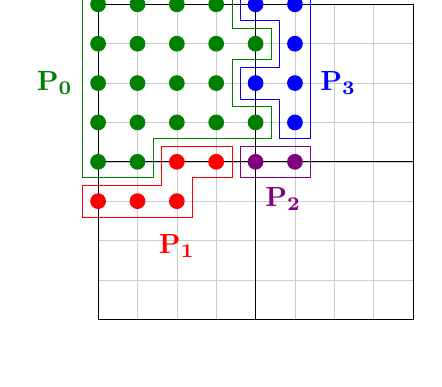
\begin{tikzpicture}%[scale=0.75]
   %
   \draw[step=0.5, black!20, very thin] (0,0) grid (4,4);
   %
   \draw (0,0) rectangle (2,2);
   \draw (2,0) rectangle (4,2);
   \draw (0,2) rectangle (2,4);
   \draw (2,2) rectangle (4,4);
   %
   \foreach \x in {0,0.5,1,1.5}
     \foreach \y in {2.5,3,3.5,4}
       \fill[fill=green!50!black] (\x, \y) circle (0.1);
   \fill[fill=green!50!black] (0,2) circle (0.1);
   \fill[fill=green!50!black] (0.5,2) circle (0.1);
   \fill[fill=green!50!black] (2,2.5) circle (0.1);
   \fill[fill=green!50!black] (2,3.5) circle (0.1);
   %
   \draw[very thin, color=green!50!black]
        (-0.2,4.2)--(1.7,4.2)--(1.7,3.7)--(2.2,3.7)--(2.2,3.3)--(1.7,3.3)--
        (1.7,2.7)--(2.2,2.7)--(2.2,2.3)--(0.7,2.3)--(0.7,1.8)--(-0.2,1.8)--
        (-0.2,4.2);
   %
   \draw[green!50!black] (-0.2,3) node[anchor=east]{$\mathbf{P_0}$};
   %
   \fill[fill=red] (1,2) circle (0.1);
   \fill[fill=red] (1.5,2) circle (0.1);
   \fill[fill=red] (0,1.5) circle (0.1);
   \fill[fill=red] (0.5,1.5) circle (0.1);
   \fill[fill=red] (1,1.5) circle (0.1);
   %
   \draw[very thin, color=red]
        (-0.2,1.7)--(0.8,1.7)--(0.8,2.2)--(1.7,2.2)--(1.7,1.8)--(1.2,1.8)--
        (1.2,1.3)--(-0.2,1.3)--(-0.2,1.7);
   %
   \draw[red] (1,1.2) node[anchor=north]{$\mathbf{P_1}$};
   %
   \fill[fill=violet] (2,2) circle (0.1);
   \fill[fill=violet] (2.5,2) circle (0.1);
   %
   \draw[very thin, color=violet]
        (1.8,2.2)--(2.7,2.2)--(2.7,1.8)--(1.8,1.8)--(1.8,2.2);
   %
   \draw[violet] (2,1.8) node[anchor=north west] {$\mathbf{P_2}$};
   %
   \fill[fill=blue] (2,4) circle (0.1);
   \fill[fill=blue] (2,3) circle (0.1);
   \fill[fill=blue] (2.5,4) circle (0.1);
   \fill[fill=blue] (2.5,3.5) circle (0.1);
   \fill[fill=blue] (2.5,3) circle (0.1);
   \fill[fill=blue] (2.5,2.5) circle (0.1);
   %
   \draw[very thin, color=blue]
     (1.8,4.2)--(2.7,4.2)--(2.7,2.3)--(2.3,2.3)--(2.3,2.8)--(1.8,2.8)--
     (1.8,3.2)--(2.3,3.2)--(2.3,3.8)--(1.8,3.8)--(1.8,4.2);
   %
   \draw[blue] (2.7,3) node[anchor=west]{$\mathbf{P_3}$};
   %
 \end{tikzpicture}

\caption{Domain partitioning: DoF of process $\mathbf{P_0}$ are marked in green
        (interior DoF in the diagonal block); the remaining DoF represent
         inter-process couplings for process $\mathbf{P_0}$ 
        (ghost DoF in the off-diagonal block)}
\label{fig:domaindecomposition}
\end{figure}

The distributed (sparse) matrix vector multiplication is given in
Algorithm~\ref{alg_mvmult}. While every process is computing its local
contribution of the matrix vector multiplication an asynchronous communication
for exchanging the ghost values is initiated. After this communication
phase has been completed, the local contributions from coupled ghost DoF are
added accordingly.
%
\begin{figure}[!ht]
  $$
  \underbrace{
  \left(
  \begin{array}{ccccc}
    ~ & ~ & ~ & ~ & ~ \\
    ~ & ~ & ~ & ~ & ~ \\
    ~ & ~ & \mathbf{P_0} & ~ & ~\\
    ~ & ~ & ~ & ~ & ~ \\
    ~ & ~ & ~ & ~ & ~
  \end{array}
  \right)
  }_{\mathrm{diagonal~block}}
  %
  \underbrace{
  \left(
  \begin{array}{c}
    {\color{green!50!black} \bullet} \\
    {\color{green!50!black} \bullet} \\
    {\color{green!50!black} \bullet} \\
    {\color{green!50!black} \bullet} \\
    {\color{green!50!black} \bullet}
  \end{array}
  \right)
  }_{\mathrm{interior}}
  %
  +
  %
  \underbrace{
  \left(
  \begin{array}{c|c|c}
    ~ & ~ & ~ \\
    ~ & ~ & ~ \\
    \mathbf{P_1} & \mathbf{P_2} & \mathbf{P_3} \\
    ~ & ~ & ~ \\
    ~ & ~ & ~
  \end{array}
  \right)
  }_{\mathrm{offdiagonal~block}}
  %
  \underbrace{
  \left(
  \begin{array}{c}
    {\color{red} \bullet} \\
    {\color{violet} \bullet} \\
    {\color{blue} \bullet} \\
    {\color{blue} \bullet}  \end{array}
  \right)
  }_{\mathrm{ghost}}
  %
  $$
\caption{Distributed matrix vector multiplication}
\label{fig:mvmult}
\end{figure}
%
\begin{algorithm}[tb]
%
\begin{algorithmic}
  \Function{distr\_mvmult}{$A, x, y$}
    \State Start asynchronous communication: exchange ghost values;
    \State $y_{\mathrm{int}} = A_{\mathrm{diag}} \, x_{\mathrm{int}}$;
    \State Synchronize communication;
    \State $y_{\mathrm{int}} =  y_{\mathrm{int}} + A_{\mathrm{offdiag}} \,
x_{\mathrm{ghost}}$;
  \EndFunction
\end{algorithmic}
\caption{Distributed matrix vector multiplication $y = Ax$}
\label{alg_mvmult}
\end{algorithm}

\subsection{Local On-Node Level}

The highly optimized BLAS 1 and 2 routines are implemented in the local
multi-platform linear algebra toolbox (lmpLAtoolbox) which is acting on each
of the subdomains. After the discretization of the PDE by means of finite
element or finite volume methods typically a large sparse linear system with
very low number of non-zeros is obtained. Therefore, the Compressed Sparse Row
(CSR) data structure \cite{templates} is the favorable sparse matrix data
format. On the NVIDIA GPU platforms we use a CUDA implementation with CSR
matrix-vector multiplication based on a scalar version as it is described in
\cite{IBM_SPMV,NVIDIA_SPMV}. Our library supports several back-ends including
multi-core CPUs, GPUs (CUDA/NVIDIA) and OpenCL (NVIDIA).

The LAtoolbox provides unified interfaces as an abstraction of the
hardware and gives easy-to-use access to the underlying heterogeneous
platforms. In this respect the application developer can utilize the
LAtoolbox without any knowledge of the hardware and the system configuration.
The final decision on which specific platform the application will be
executed can be taken at run time. A data parallel model is used for the
parallelization of the basic BLAS 1 and 2 routines which by their nature provide
fine-grained parallelism. From a theoretical point of view the data parallel
model results in good load balancing and scalability across several computing
units. These expectations have been confirmed by our practical experiments
across a variety of platforms and systems.

\begin{figure}[ht]
\centering
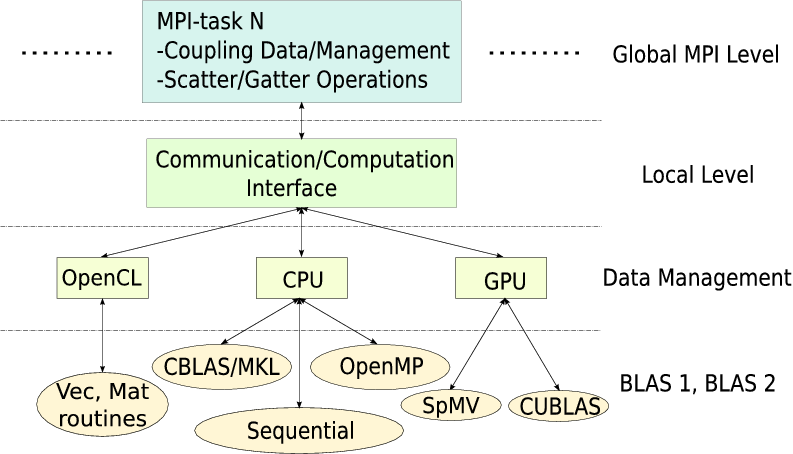
\includegraphics[scale=0.5]{./fig/LAtoolbox_new_3.png}
\caption{Structure of the lmpLAtoolbox and LAtoolbox
for distributed computation and node-level computation across several devices
in a homogeneous and heterogeneous environment.} 
\label{latoolbox}
\end{figure}

The layered structure and organization of both the LAtoolbox and the
lmpLAtoolbox is depicted in Figure~\ref{latoolbox}. It shows a high-level
view of distributed communication and computation across nodes and the
node-level computation across several devices in a heterogeneous environment.

A cross-platform makefile generator (cmake) identifies all software
libraries (i.e.~OpenMP, CUDA, MKL, and etc) available on the underlying
computing platform. After compilation the decision of final platform can be
taken at run-time e.g.~by providing information in a configuration file or from
user input. All data structures (matrices and vectors) are distributed
or offloaded accordingly. On a lean platform like a netbook or even a smartphone
the project and all modules can be used in their sequential version.
Within this setting there is further room for autotuning mechanisms, e.g.~when
several devices are available.

The code fragment in Listing~\ref{lmpLAtoolbox} exemplifies handling of the
lmpLAtoolbox. It details declaration of two vectors and a matrix. The CPU
performs all input and output operations. To this end, the CPU matrix type is
declared. Later conversion between two different platforms is based on a
copy-like function. For avoiding unnecessary transfers to the same device a
simple platform check is typically used.

The PCIe bus between host and device is a known bottleneck for attached
accelerators. In particular, bandwidth limitations occur for updates of
inter-process couplings between subdomains kept on different devices.
Advanced data packaging and transfer techniques are utilized for
mitigation of delays due to these inevitable cross-device data transfers.
The underlying idea for maximized throughput is to manage and reorganize
irregular data structures on the host CPUs and to transfer repackaged data in
huge and continuous buffers to the accelerators. 


Due to the full abstraction within the libraries there is limited or no
access to the platform-specific data buffers. In certain cases -- e.g.~for
nested loop iterations or irregular data access patterns -- there is the option
for defining device-specific data structures (vectors and matrices) with
direct access to all data buffers.

\lstinputlisting[language=C++, label=lmpLAtoolbox, 
caption=Example code for lmpLAtoolbox]{lmplatoolbox.cc}

Due to the modular setup and the consistent structure, the lmpLAtoolbox can be
used as a standalone library independently of HiFlow${}^3$. It offers a complete
and unified interface for many hardware platforms. Hence, the LAtoolbox not only
offers fined-grained parallelism but also flexible utilization and
cross-platform portability.

Theoretical details as well as benchmarks on different platforms of the
preconditioners with impact on the solution procedure can be found in
\cite{Lukarski2012}. 

\subsection{Different Backends on the Global-level}

The global platform abstracted vectors and matrices have to be declared as
pointers to the base class and initiated via the \verb'init_platform_vec<>()' and
\verb'init_platform_mat<>()' init functions. Always the platform
vectors/matrices have to be allocated together with the corresponding CPU
vectors/matrices.  If the vectors/matrices are set to be a CPU type -- the
pointers (\verb'dev_' device-pointers) refer to the CPU objects. An example
for the allocation can be found in Listing~\ref{LAtoolbox-var}.

\lstinputlisting[language=C++, label=LAtoolbox-var, 
caption=Platform abstracted vectors/matrices declaration in LAtoolbox]{latoolbox-var.cc}

The pair of vectors/matrices (i.e.~for CPU and platform-specific) are needed
mainly for the assembling procedure -- it is available only for CPU-based
objects, see Listing~\ref{LAtoolbox-assemb}. After the assembling procedure
the data are copied to the platform-specific objects -- in case of CPU
vectors/matrices the copy functions do not call itself.

\lstinputlisting[language=C++, label=LAtoolbox-assemb, 
caption=Assembling for pPlatform abstracted vectors/matrices]{latoolbox-assemb.cc}

On the other side, the preconditioners and the solver can work only with the
abstracted objects (i.e.~pointers to the base class). However, there is one
more trick for deploying some of the preconditioners -- it might need to
permute the stiffness matrix. Due to the couplings, this step is performed on
the global level with the permutation function in the DoF module. An example
for building different preconditioners is shown in
Listing~\ref{LAtoolbox-precond-solver}. The linear solver works directly with
the base class of the vectors/matrices objects -- for post-processing the data
needs to be copy back from the device. 

\lstinputlisting[language=C++, label=LAtoolbox-precond-solver, 
caption=Block-preconditioners and solver with platform abstracted
vectors/matrices]{latoolbox-precond-solver.cc} 


\subsection{Parameter File}\index{parameter file}\label{sectionparameter file}

The needed parameters are initialized in the paramter file
convdiff\_benchmark.xml.

The \verb'Platform' can be \verb'CPU', \verb'GPU' or \verb'OpenCL'. The
possible matrix implementations are \verb'MKL' and \verb'OPENMP' for the CPU
platform; \verb'SCALAR' and \verb'SCALAR_TEX' for the GPU (NVIDIA CUDA); and
\verb'OpenCL' for the \verb'OpenCL' GPU NVIDIA devices. The possible vector
implementations are \verb'BLAS', \verb'MKL' and \verb'OPENMP' for the CPU
platform; \verb'BLAS' for the GPU (NVIDIA CUDA); and \verb'OpenCL' for the
\verb'OpenCL' backend.
The parameters for the preconditioners and solvers can be found in the
Listing~\ref{LAtoolbox-precond-solver} -- see file \verb'convdiff_benchmark.xml'. 

\begin{lstlisting}[language=XML, basicstyle={\footnotesize, \ttfamily},
    keywordstyle=\color{blue}, numbers=none, tabsize=4] 
<Param>
  <Model>
    <nu>1./37.</nu>
    <beta1>1.</beta1>
    <beta2>1.</beta2>
    <beta3>1.</beta3>
  </Model>
  <Mesh>
    <Filename>unit_square.inp</Filename>
    <RefinementLevel>4</RefinementLevel>
  </Mesh>
  <LinearAlgebra>
    <Platform>CPU</Platform>
    <MatrixImplementation>Naive</MatrixImplementation>
    <VectorImplementation>Naive</VectorImplementation>
    <MatrixFormat>CSR</MatrixFormat>
    <MatrixFreePrecond>ILU</MatrixFreePrecond>
    <ILU2Param1>1</ILU2Param1>
    <ILU2Param2>2</ILU2Param2>
  </LinearAlgebra>
  <FiniteElements>
    <Degree>3</Degree>
  </FiniteElements>
  <LinearSolver>
    <Name>GMRES</Name>
    <MaxIterations>10000</MaxIterations>
    <AbsTolerance>1.e-14</AbsTolerance>
    <RelTolerance>1.e-8</RelTolerance>
    <DivTolerance>1.e6</DivTolerance>
    <SizeBasis>50</SizeBasis>
    <Method>RightPreconditioning</Method>
    <UseILUPP>1</UseILUPP>
  </LinearSolver>
  <ILUPP>
    <PreprocessingType>0</PreprocessingType>
    <PreconditionerNumber>1010</PreconditionerNumber>
    <MaxMultilevels>20</MaxMultilevels>
    <MemFactor>0.8</MemFactor>
    <PivotThreshold>1.75</PivotThreshold>
    <MinPivot>0.01</MinPivot>
  </ILUPP>
  <Output>
    <LogFilename>info_conv_diff.log</LogFilename>
  </Output>
</Param>
\end{lstlisting}

\section{GPU Clusters}

The LAtoolbox can run on GPU cluster using MPI. Details can be found in the
Poisson Tutorial.

You can change the number of GPU devices per node in the file
\verb'platform_management.cc' (in \verb'src/linear_algebra/lmp/'). The
variable \verb'num_gpu_per_node' describes the number of GPU devices that 
are availbe per node.

To obtain good scalability the mesh partitioning should provide minimum
communication pattern -- the ghost nodes should be as small as possible in
order to minimize the communication over the PCI-E and network. Please note
that the local preconditioners are applied in a block-Jacobi way and this
will lead to different performance behavior of the linear solver for different
number of MPI processes. To measure the pure scalability of cluster, you should
use either no preconditioner or Jacobi type of preconditioner. Details can be 
found in \cite{HSLW2010,Lukarski2012}.


\newpage
%\appendix

\bibliography{tutorials_bib}
\bibliographystyle{plain}

\printindex

\end{document}
